\documentclass[12pt,a4paper]{article}
\usepackage[utf8]{inputenc}
\usepackage[T1]{fontenc}
\usepackage[polish]{babel}
\usepackage{float}
\usepackage{cite}

\usepackage{pgfplots}
\usepackage{pgfplotstable}
\pgfplotsset{compat=newest}

\begin{document}

\title{[PSZT] PZ.U17 - Marketing bankowy}
\author{Adrian Brodzik \and Jakub Górka}
\maketitle

\section*{Zadanie}
Porównać algorytmy regresji logistycznej i XGBoost.

\section*{Teza}
\textbf{Efektywność regresji logistycznej i XGBoost jest równa dla problemu ustalenia potencjalnych klientów lokat bankowych pewnej portugalskiej instytucji finansowej.}

\section*{Analiza danych}
Źródło danych: \texttt{https://archive.ics.uci.edu/ml/datasets/Bank+Marketing}
\\
Plik danych: \texttt{bank-additional-full.csv}
\\
Opis danych: \texttt{bank-additional-names.txt}

\section*{Eksperyment}
Dane są ładowane z pliku \texttt{bank-additional-full.csv} do pamięci za pomocą modułu \texttt{pandas}.
\\
\\
Wartości kolumny celu \texttt{y} są mapowane na $0$ dla wartości \texttt{no}, albo $1$ dla wartości \texttt{yes}. Następnie wartości kolumn kategorycznych są jednoznacznie mapowane na liczby całkowite dodatnie. Gdyby model był zapisany i uruchomiony na nowych danych, to wartości danych powinny być dokładnie tak zakodowane, jak podczas procesu uczenia się modelu. Natomiast dane, które nigdy wcześniej się nie pojawiły są kodowane na wartość wyrażenia \texttt{\_\_UNKNOWN\_\_}. Na koniec usuwane są kolumny niepotrzebne (w zależności od wykonywanego eksperymentu).
\\
\\
Do podziału danych wykorzystany jest proces k-krotnej walidacji z modułu \texttt{scikit-learn}. Ponadto dane są rozłożone równomiernie ze względu na wartość kolumny celu \texttt{y} (ang. \textit{stratified k-fold}).
\\
\\
W każdej z $k$ iteracji generowane są dwa zbiory danych: treningowy oraz walidacyjny. Zbiór treningowy służy do uczenia modelu \texttt{LogisticRegression} z modułu \texttt{scikit-learn} albo \texttt{XGBRegressor} z modułu \texttt{XGBoost}. Zbiór walidacyjny służy do oceny nauczonego modelu, np. za pomocą \texttt{roc\_auc\_score} z modułu \texttt{scikit-learn}. ROC-AUC określa w jakim stopniu nauczony model jest w stanie rozpoznać daną klasę.

\section*{Hiperparametry}
Do automatycznego strojenia parametrów wykorzystano moduł \texttt{hyperopt}, a w szczególności estymator jądrowy gęstości (ang. \textit{Tree-structured Parzen Estimator}).
\\
\\
Dla regresji logistycznej przeszukano następujące parametry:
\begin{itemize}
	\item tol - tolerance for stopping criteria
	\item C - inverse of regularization strength
	\item fit\_intercept - specifies if a constant should be added to the decision function
	\item class\_weight - weights associated with classes
	\item solver - algorithm to use in the optimization problem
	\item max\_iter - maximum number of iterations taken for the solvers to converge
	\item warm\_start
\end{itemize}
Dla XGBoost przeszukano następujące parametry:
\begin{itemize}
	\item n\_estimators
	\item max\_depth
	\item learning\_rate
	\item booster
	\item tree\_method
	\item gamma
	\item subsample
	\item colsample\_bytree
	\item colsample\_bylevel
	\item colsample\_bynode
	\item reg\_alpha
	\item reg\_lambda
	\item scale\_pos\_weight
\end{itemize}

\pgfplotstableread{
	X	Y
	2	78.69714909632302
	3	78.66706102134483
	4	78.67094831360176
	5	78.65894483912202
	6	78.67538476795796
	7	78.63251478833636
	8	78.67570483656661
	9	78.68297518084827
	10	78.66307845322866
	11	78.6612037183697
	12	78.67152659420497
	13	78.69409588069043
	14	78.66424887897095
	15	78.67461243178607
}\datatableA

\pgfplotstableread{
	X	Y
	2	80.45327377695086
	3	80.44886331500206
	4	80.58865903318451
	5	80.47481124606423
	6	80.71345737170446
	7	80.57273195610956
	8	80.60197838197677
	9	80.75462585435221
	10	80.6557763109069
	12	80.67750282856588
	15	80.67771125986073
}\datatableB

\section*{Wyniki}
\begin{figure}[H]
	\centering
	\begin{tikzpicture}
	\begin{axis}[
		xlabel=k,
		ylabel=average ROC AUC (\%),
		grid=both,
		xmin=2,
		ymin=78.63,
		xmax=15,
		ymax=78.7,
		scale=1.5
	]
	\addplot [only marks, red] table {\datatableA};
	\end{axis}
	\end{tikzpicture}
	\caption{\textbf{Regresja logistyczna i k-krotna walidacja.} Wyższa ocena świadczy o efektywniejszej klasyfikacji.}
\end{figure}

\begin{figure}[H]
	\centering
	\begin{tikzpicture}
	\begin{axis}[
		xlabel=k,
		ylabel=average ROC AUC (\%),
		grid=both,
		xmin=2,
		ymin=80.4,
		xmax=15,
		ymax=80.7,
		scale=1.5
	]
	\addplot [only marks, blue] table {\datatableB};
	\end{axis}
	\end{tikzpicture}
	\caption{\textbf{XGBoost i k-krotna walidacja.} Wyższa ocena świadczy o efektywniejszej klasyfikacji.}
\end{figure}

\begin{figure}[H]
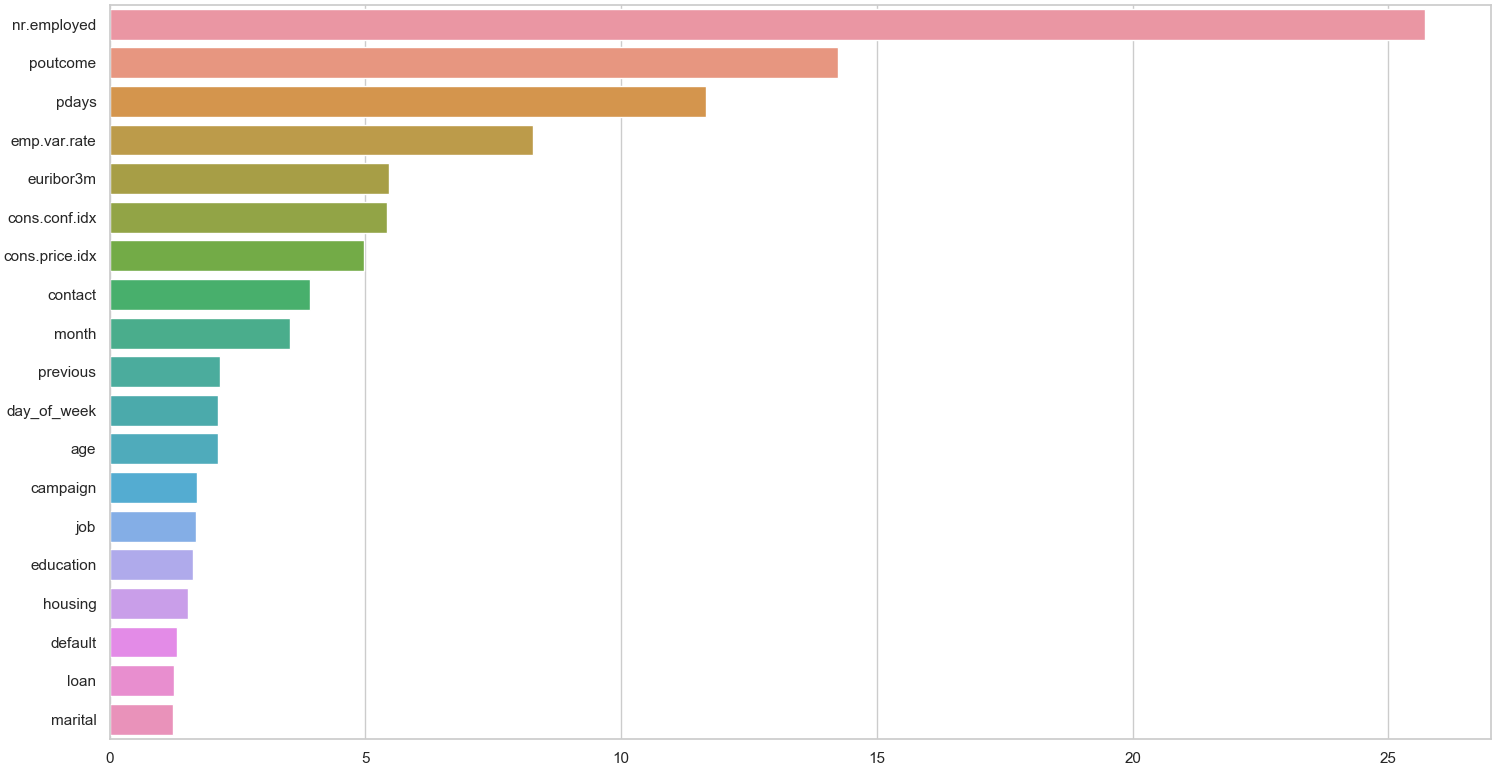
\includegraphics[scale=0.35]{features.png}
\caption{\textbf{Najważniejsze atrybuty wg XGBoost.}}
\end{figure}

\section*{Dyskusja}
Wyższa wartość $k$ w procesie k-krotnej walidacji nie oznacza, że klasyfikator będzie efektywniejszy. Zbiór treningowy jest proporcjonalnie większy, ale zbiór walidacyjny jest proporcjonalnie mniejszy. Ciężko jest wykryć przeuczenie modelu, mając zbyt mały zbiór walidacyjny.

\section*{Wnioski}
Teza została potwierdzona.

\nocite{*}
\bibliographystyle{plain}
\bibliography{Raport}{}

\end{document}